\documentclass{standalone}
\usepackage{tikz}
\usetikzlibrary{patterns, positioning}


\begin{document}
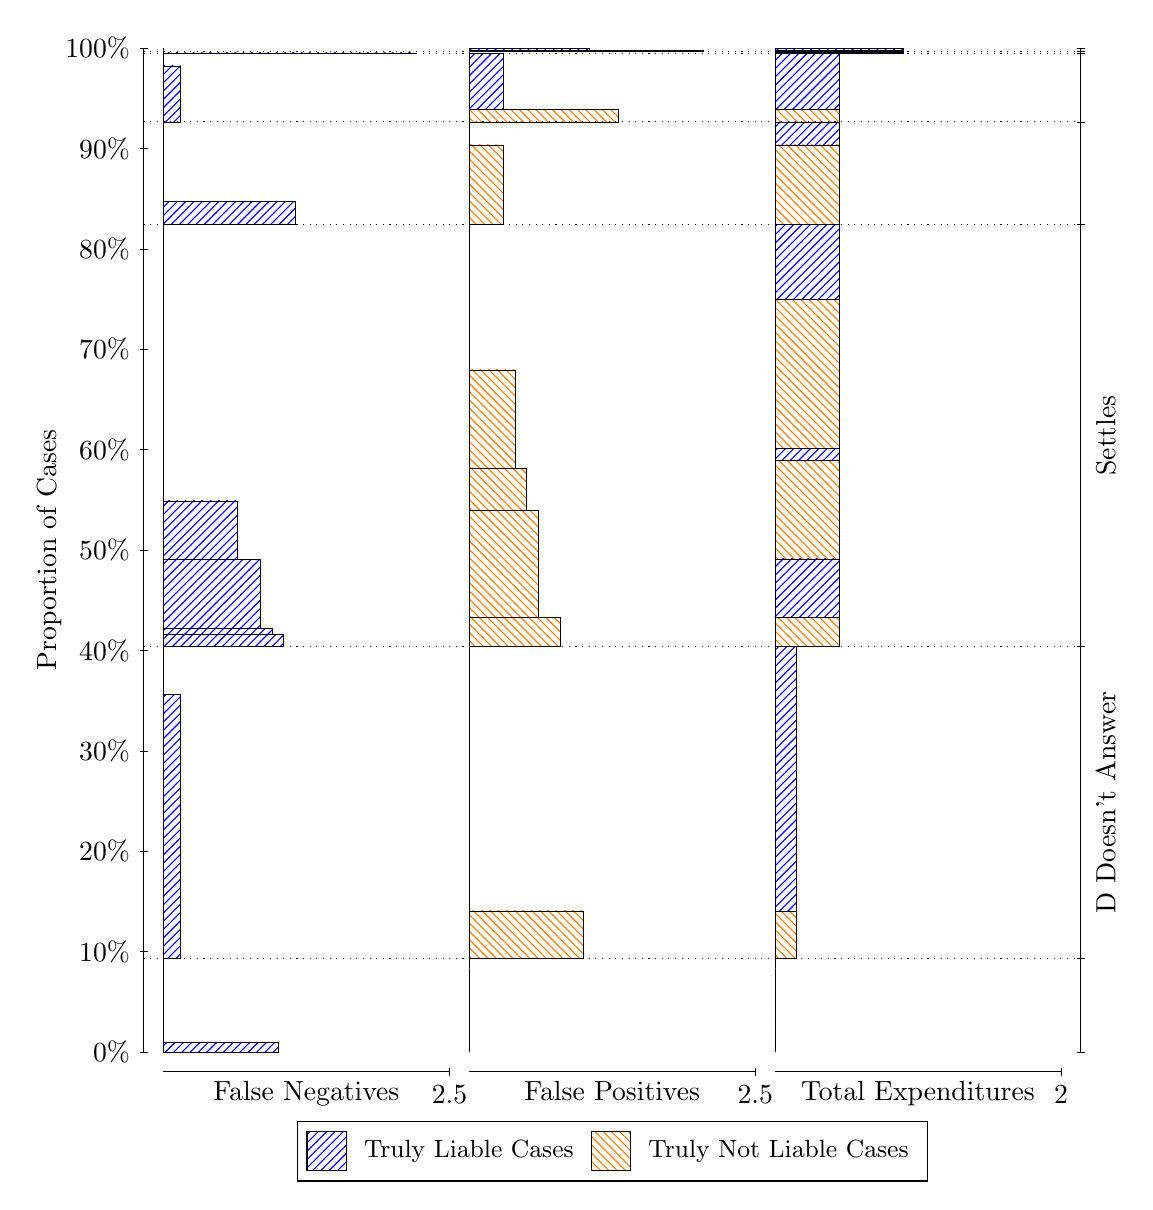
\begin{tikzpicture}
\draw[black, very thin] (1.5,1.75) -- (1.5,14.5);
\node[rotate=90, text=black, anchor=center] at (0.3, 8.125) {Proportion of Cases};
\draw[black, very thin] (1.45,1.75) -- (1.55,1.75);
\node[text=black, anchor=east] at (1.45, 1.75) {0\%};
\draw[black, very thin] (1.45,3.025) -- (1.55,3.025);
\node[text=black, anchor=east] at (1.45, 3.025) {10\%};
\draw[black, very thin] (1.45,4.3) -- (1.55,4.3);
\node[text=black, anchor=east] at (1.45, 4.3) {20\%};
\draw[black, very thin] (1.45,5.575) -- (1.55,5.575);
\node[text=black, anchor=east] at (1.45, 5.575) {30\%};
\draw[black, very thin] (1.45,6.85) -- (1.55,6.85);
\node[text=black, anchor=east] at (1.45, 6.85) {40\%};
\draw[black, very thin] (1.45,8.125) -- (1.55,8.125);
\node[text=black, anchor=east] at (1.45, 8.125) {50\%};
\draw[black, very thin] (1.45,9.4) -- (1.55,9.4);
\node[text=black, anchor=east] at (1.45, 9.4) {60\%};
\draw[black, very thin] (1.45,10.675) -- (1.55,10.675);
\node[text=black, anchor=east] at (1.45, 10.675) {70\%};
\draw[black, very thin] (1.45,11.95) -- (1.55,11.95);
\node[text=black, anchor=east] at (1.45, 11.95) {80\%};
\draw[black, very thin] (1.45,13.225) -- (1.55,13.225);
\node[text=black, anchor=east] at (1.45, 13.225) {90\%};
\draw[black, very thin] (1.45,14.5) -- (1.55,14.5);
\node[text=black, anchor=east] at (1.45, 14.5) {100\%};

\draw[black, very thin] (13.4,1.75) -- (13.4,14.5);
\draw[black, very thin] (13.35,1.75) -- (13.45,1.75);
\node[anchor=west] at (13.35, 1.75) {};
\draw[black, very thin] (13.35,2.9362) -- (13.45,2.9362);
\node[anchor=west] at (13.35, 2.9362) {};
\draw[black, very thin] (13.35,6.8976) -- (13.45,6.8976);
\node[anchor=west] at (13.35, 6.8976) {};
\draw[black, very thin] (13.35,12.264) -- (13.45,12.264);
\node[anchor=west] at (13.35, 12.264) {};
\draw[black, very thin] (13.35,13.563) -- (13.45,13.563);
\node[anchor=west] at (13.35, 13.563) {};
\draw[black, very thin] (13.35,14.427) -- (13.45,14.427);
\node[anchor=west] at (13.35, 14.427) {};
\draw[black, very thin] (13.35,14.457) -- (13.45,14.457);
\node[anchor=west] at (13.35, 14.457) {};
\draw[black, very thin] (13.35,14.5) -- (13.45,14.5);
\node[anchor=west] at (13.35, 14.5) {};

\draw[black, very thin, pattern color=blue, pattern=north east lines] (1.75,1.75) rectangle (3.2033,1.8748);
\draw[black, very thin, pattern color=orange, pattern=north west lines] (1.75,1.8748) rectangle (1.75,2.9362);
\draw[black, very thin, pattern color=blue, pattern=north east lines] (1.75,2.9362) rectangle (1.968,6.2921);
\draw[black, very thin, pattern color=orange, pattern=north west lines] (1.75,6.2921) rectangle (1.75,6.8976);
\draw[black, very thin, pattern color=blue, pattern=north east lines] (1.75,6.8976) rectangle (3.276,7.0505);
\draw[black, very thin, pattern color=blue, pattern=north east lines] (1.75,7.0505) rectangle (3.1307,7.1259);
\draw[black, very thin, pattern color=blue, pattern=north east lines] (1.75,7.1259) rectangle (2.9853,8.0046);
\draw[black, very thin, pattern color=blue, pattern=north east lines] (1.75,8.0046) rectangle (2.6947,8.7484);
\draw[black, very thin, pattern color=orange, pattern=north west lines] (1.75,8.7484) rectangle (1.75,12.264);
\draw[black, very thin, pattern color=blue, pattern=north east lines] (1.75,12.264) rectangle (3.4213,12.555);
\draw[black, very thin, pattern color=orange, pattern=north west lines] (1.75,12.555) rectangle (1.75,13.563);
\draw[black, very thin, pattern color=blue, pattern=north east lines] (1.75,13.563) rectangle (1.968,14.272);
\draw[black, very thin, pattern color=orange, pattern=north west lines] (1.75,14.272) rectangle (1.75,14.427);
\draw[black, very thin, pattern color=blue, pattern=north east lines] (1.75,14.427) rectangle (4.9473,14.439);
\draw[black, very thin, pattern color=orange, pattern=north west lines] (1.75,14.439) rectangle (1.75,14.457);
\draw[black, very thin, pattern color=orange, pattern=north west lines] (1.75,14.457) rectangle (1.75,14.47);
\draw[black, very thin, pattern color=blue, pattern=north east lines] (1.75,14.47) rectangle (1.75,14.5);
\draw[black, very thin, pattern color=orange, pattern=north west lines] (5.6333,1.75) rectangle (5.6333,2.8114);
\draw[black, very thin, pattern color=blue, pattern=north east lines] (5.6333,2.8114) rectangle (5.6333,2.9362);
\draw[black, very thin, pattern color=orange, pattern=north west lines] (5.6333,2.9362) rectangle (7.0867,3.5417);
\draw[black, very thin, pattern color=blue, pattern=north east lines] (5.6333,3.5417) rectangle (5.6333,6.8976);
\draw[black, very thin, pattern color=orange, pattern=north west lines] (5.6333,6.8976) rectangle (6.796,7.2681);
\draw[black, very thin, pattern color=orange, pattern=north west lines] (5.6333,7.2681) rectangle (6.5053,8.6266);
\draw[black, very thin, pattern color=orange, pattern=north west lines] (5.6333,8.6266) rectangle (6.36,9.1641);
\draw[black, very thin, pattern color=orange, pattern=north west lines] (5.6333,9.1641) rectangle (6.2147,10.413);
\draw[black, very thin, pattern color=blue, pattern=north east lines] (5.6333,10.413) rectangle (5.6333,12.264);
\draw[black, very thin, pattern color=orange, pattern=north west lines] (5.6333,12.264) rectangle (6.0693,13.271);
\draw[black, very thin, pattern color=blue, pattern=north east lines] (5.6333,13.271) rectangle (5.6333,13.563);
\draw[black, very thin, pattern color=orange, pattern=north west lines] (5.6333,13.563) rectangle (7.5227,13.717);
\draw[black, very thin, pattern color=blue, pattern=north east lines] (5.6333,13.717) rectangle (6.0693,14.427);
\draw[black, very thin, pattern color=orange, pattern=north west lines] (5.6333,14.427) rectangle (5.6333,14.445);
\draw[black, very thin, pattern color=blue, pattern=north east lines] (5.6333,14.445) rectangle (5.6333,14.457);
\draw[black, very thin, pattern color=orange, pattern=north west lines] (5.6333,14.457) rectangle (8.6127,14.47);
\draw[black, very thin, pattern color=blue, pattern=north east lines] (5.6333,14.47) rectangle (7.1593,14.5);
\draw[black, very thin, pattern color=orange, pattern=north west lines] (9.5167,1.75) rectangle (9.5167,2.8114);
\draw[black, very thin, pattern color=blue, pattern=north east lines] (9.5167,2.8114) rectangle (9.5167,2.9362);
\draw[black, very thin, pattern color=orange, pattern=north west lines] (9.5167,2.9362) rectangle (9.7892,3.5417);
\draw[black, very thin, pattern color=blue, pattern=north east lines] (9.5167,3.5417) rectangle (9.7892,6.8976);
\draw[black, very thin, pattern color=orange, pattern=north west lines] (9.5167,6.8976) rectangle (10.334,7.2681);
\draw[black, very thin, pattern color=blue, pattern=north east lines] (9.5167,7.2681) rectangle (10.334,8.0119);
\draw[black, very thin, pattern color=orange, pattern=north west lines] (9.5167,8.0119) rectangle (10.334,9.2607);
\draw[black, very thin, pattern color=blue, pattern=north east lines] (9.5167,9.2607) rectangle (10.334,9.4136);
\draw[black, very thin, pattern color=orange, pattern=north west lines] (9.5167,9.4136) rectangle (10.334,11.31);
\draw[black, very thin, pattern color=blue, pattern=north east lines] (9.5167,11.31) rectangle (10.334,12.264);
\draw[black, very thin, pattern color=orange, pattern=north west lines] (9.5167,12.264) rectangle (10.334,13.271);
\draw[black, very thin, pattern color=blue, pattern=north east lines] (9.5167,13.271) rectangle (10.334,13.563);
\draw[black, very thin, pattern color=orange, pattern=north west lines] (9.5167,13.563) rectangle (10.334,13.717);
\draw[black, very thin, pattern color=blue, pattern=north east lines] (9.5167,13.717) rectangle (10.334,14.427);
\draw[black, very thin, pattern color=orange, pattern=north west lines] (9.5167,14.427) rectangle (11.152,14.445);
\draw[black, very thin, pattern color=blue, pattern=north east lines] (9.5167,14.445) rectangle (11.152,14.457);
\draw[black, very thin, pattern color=orange, pattern=north west lines] (9.5167,14.457) rectangle (11.152,14.47);
\draw[black, very thin, pattern color=blue, pattern=north east lines] (9.5167,14.47) rectangle (11.152,14.5);
\draw[black, dotted] (1.5,2.9362) -- (13.4,2.9362);
\draw[black, dotted] (1.5,6.8976) -- (13.4,6.8976);
\draw[black, dotted] (1.5,12.264) -- (13.4,12.264);
\draw[black, dotted] (1.5,13.563) -- (13.4,13.563);
\draw[black, dotted] (1.5,14.427) -- (13.4,14.427);
\draw[black, dotted] (1.5,14.457) -- (13.4,14.457);
\draw[black, very thin] (1.75,1.5) -- (5.3833,1.5);
\node[text=black, anchor=north] at (3.5667, 1.5) {False Negatives};
\draw[black, very thin] (5.3833,1.45) -- (5.3833,1.55);
\node[text=black, anchor=north] at (5.3833, 1.45) {2.5};

\draw[black, very thin] (5.6333,1.5) -- (9.2667,1.5);
\node[text=black, anchor=north] at (7.45, 1.5) {False Positives};
\draw[black, very thin] (9.2667,1.45) -- (9.2667,1.55);
\node[text=black, anchor=north] at (9.2667, 1.45) {2.5};

\draw[black, very thin] (9.5167,1.5) -- (13.15,1.5);
\node[text=black, anchor=north] at (11.333, 1.5) {Total Expenditures};
\draw[black, very thin] (13.15,1.45) -- (13.15,1.55);
\node[text=black, anchor=north] at (13.15, 1.45) {2};


\node[text=black, centered, rotate=90] at (13.72, 4.9169) {D Doesn't Answer};
\node[text=black, centered, rotate=90] at (13.72, 9.5806) {Settles};





\draw (7.449999999999999,1.5) node[draw=none] (baseCoordinate) {};
\begin{scope}[align=center]
        \matrix[scale=0.5, draw=black, below=0.5cm of baseCoordinate, nodes={draw}, column sep=0.1cm]{
            \node[rectangle, draw, minimum width=0.5cm, minimum height=0.5cm, pattern color=blue, pattern=north east lines] {}; &
            \node[draw=none, font=\small, text=black] (B) {Truly Liable Cases}; &
            \node[rectangle, draw, minimum width=0.5cm, minimum height=0.5cm, pattern color=orange, pattern=north west lines] {}; &
            \node[draw=none, font=\small, text=black] (B) {Truly Not Liable Cases}; \\
            };
\end{scope}

\end{tikzpicture}
\end{document}